\section{Experimental Results}
\label{sec:results}

% does the complete system actually produce good hardware, generalize, remain valid, and beat alternatives?

We organize the evaluation around four questions:
(1) does the direct policy produce high-quality feasible designs on held-out and external kernels;
(2) does changing the deployment request move the synthesized design in the intended direction;
(3) does correctly aligned compiler memory improve the policy beyond task-specific fine-tuning and a generic side channel; and
(4) how does the resulting policy compare with LLM and DSE baselines in validity, QoR, and online HLS cost?


\subsection{End-to-End Evaluation and Generalization}
\label{subsec:salt-evaluation}


\begin{figure*}[t]
    \centering
    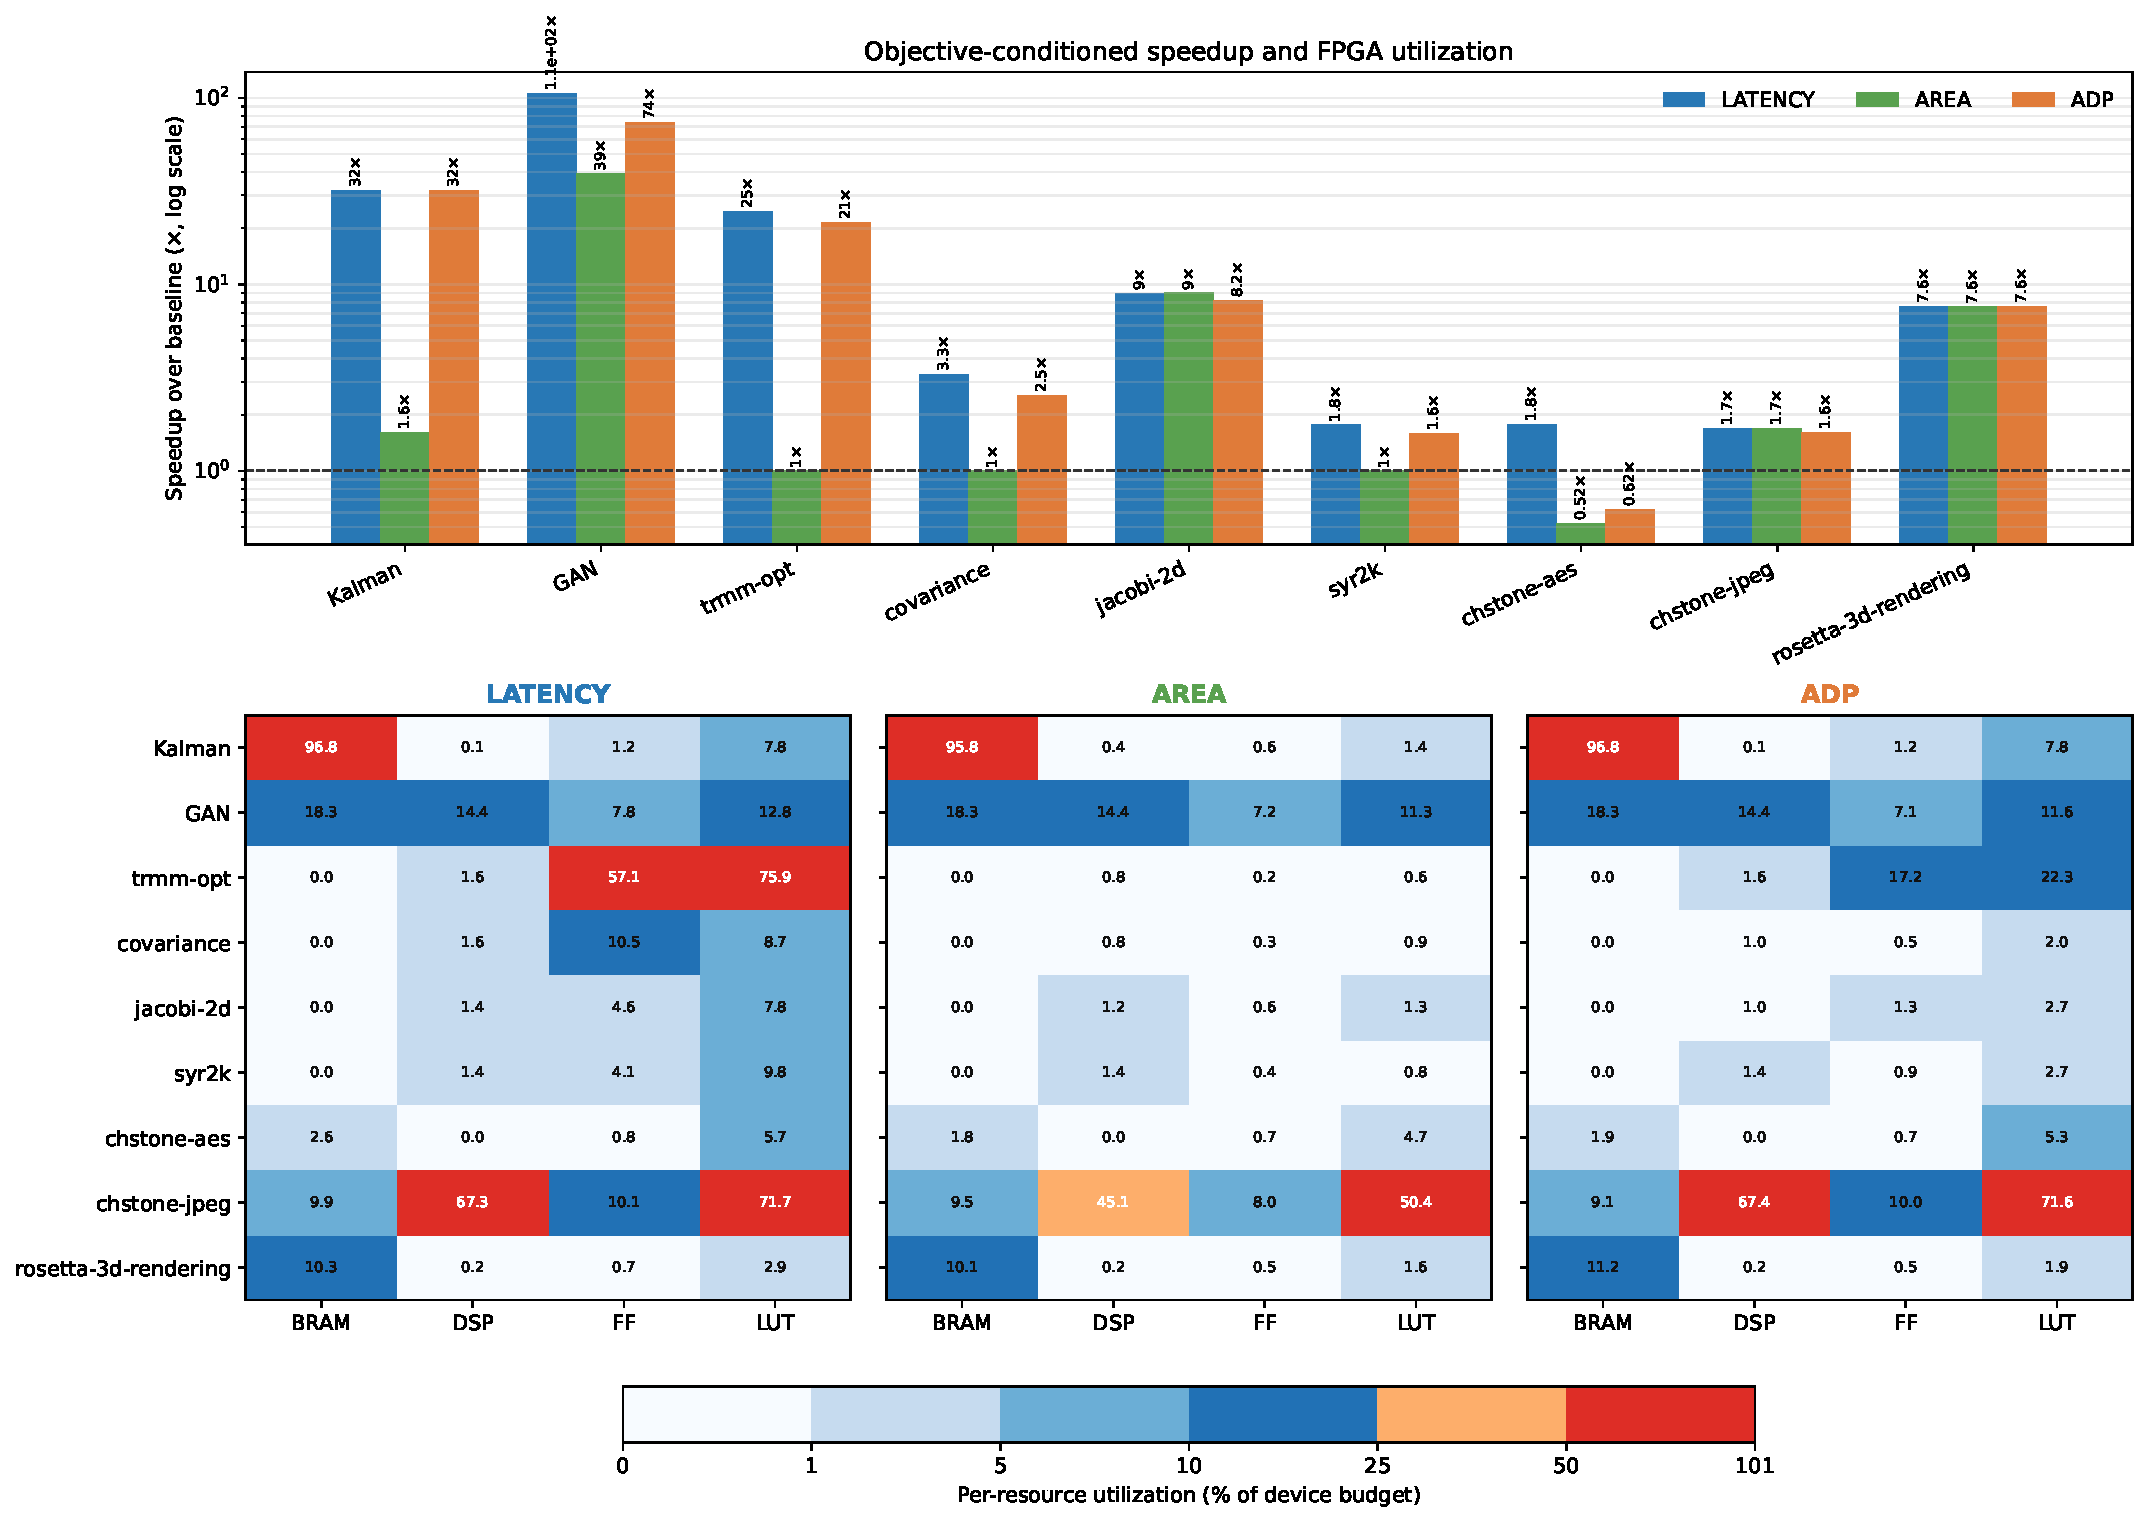
\includegraphics[
        width=0.96\textwidth
    ]{figures/04_Experimental/objective_speedup_resource_overview.pdf}
    \caption{
        \textbf{Objective-conditioned synthesized QoR across the evaluation suite.}
        Top: speedup over the corresponding pragma-free Vitis baseline for the
        latency-, area-, and ADP-oriented SALT-HLS policies.
        Bottom: per-resource BRAM, DSP, FF, and LUT utilization as a percentage
        of the target-device capacity for each objective.
        The results show that objective conditioning produces distinct
        performance--resource operating points rather than a single
        target-invariant directive policy.
    }
    \Description{
        Objective-conditioned SALT-HLS results across nine kernels.
        The upper panel compares latency, area, and ADP speedups over
        pragma-free Vitis on a logarithmic scale. Three lower heatmaps
        report BRAM, DSP, FF, and LUT utilization for the corresponding
        objective-specific designs.
    }
    \label{fig:objective-qor-overview}
\end{figure*}


\paragraph{End-to-end objective-conditioned QoR.}
Figure~\ref{fig:objective-qor-overview} evaluates the complete
SALT-HLS deployment path rather than prediction accuracy in
isolation. For every kernel, we fix the target (ZCU104/10\,ns),
resource capacity, source code, and legal directive action space,
and vary only the requested optimization policy. The latency, area,
and ADP models each emit one complete directive configuration
without online HLS feedback; the resulting design is synthesized
once to obtain the reported QoR. This setup therefore isolates two
questions central to SALT-HLS: whether a learned policy transfers
across heterogeneous workloads, and whether changing the objective
actually produces a different hardware optimization strategy rather
than a common directive template. All 27 objective-conditioned
designs reported in the figure satisfy the device resource limits.

Across the nine kernels, the latency policy achieves a
7.73$\times$ geometric-mean speedup over pragma-free Vitis.
The area policy reduces the suite-average area proxy $A$ from
14.61\% to 8.09\%---a 44.6\% reduction relative to the
latency policy---while retaining a 2.50$\times$ geometric-mean
speedup. ADP occupies the intended intermediate regime, reaching
6.16$\times$ at 10.88\% average $A$. The separation is expressed
primarily through FF and LUT consumption: their average utilization
falls from 10.76\%/22.57\% under latency optimization to
2.06\%/8.12\% under area optimization, whereas average BRAM
changes little. This is consistent with several workloads having a
memory footprint that forms a largely objective-independent floor,
while replication, scheduling, and control logic provide more freedom
for trading throughput against area.

The per-kernel spread also shows why optimization headroom cannot be
inferred from program size alone. GAN starts from a resource-light
baseline and exposes abundant regular compute parallelism, allowing
the latency policy to reach 105.39$\times$. Kalman represents the
opposite regime: its pragma-free implementation already consumes
97.1\% of ZCU104 BRAM, yet SALT-HLS reaches 31.81$\times$ while
using 96.8\% BRAM, i.e., the gain cannot be explained by simply
allocating more memory. Conversely, TRMM exposes only three directive
sites but reaches 24.62$\times$, whereas the structurally larger JPEG
kernel exposes 21 sites yet reaches only 1.70$\times$. Thus, the
number of available decisions is a poor proxy for achievable QoR:
the decisive factor is whether the program's dependence and memory
structure permits a few transformations to unlock useful parallelism.
The variation across Covariance (3.29$\times$), Jacobi-2D
(8.97$\times$), SYR2K (1.77$\times$), and TRMM
(24.62$\times$) makes the same point even within the regular
PolyBench class.

\paragraph{Directive-level policy specialization.}
The synthesized QoR differences correspond to substantial changes in
the directives themselves. Across the fixed 65 loop and 20 array
action sites, the latency policy enables pipelining at 50.8\% of loop
sites, non-trivial unrolling at 44.6\%, and array partitioning at
80.0\% of array sites. The area policy reduces these rates to
30.8\%, 12.3\%, and 40.0\%, respectively, and leaves both
pipeline and unroll disabled at 56.9\% of loop sites. ADP again lies
between the two, with 43.1\% pipelined loops, 32.3\% unrolled loops,
and 75.0\% partitioned arrays. Overall, the latency and area policies
select different complete directive assignments at 44 of the 85
action sites (51.8\%). Because the action locations and legal domains
are identical across objectives, this difference reflects learned
policy specialization rather than a change in the available search
space.

The specialization is microarchitecturally coherent rather than merely
statistical. On GAN, for example, the latency policy couples cyclic
partition factors of 15 and 25 on the hidden-layer buffers with
unroll factors of 30, 30, 15, and 25, reaching 105.39$\times$.
ADP narrows the corresponding banking to 5 and 5 and the unrolling
to 10, 10, 5, and 5, reaching 74.06$\times$; the area policy
reduces banking to factor 2 and removes explicit unrolling, reaching
39.10$\times$ with lower hardware cost. TRMM exhibits the same
ordering more sharply: the latency policy combines $20\times$
unrolling with two pipelined loops (24.62$\times$, $A=33.66\%$),
ADP uses $5\times$ unrolling and one pipeline
(21.48$\times$, $A=10.28\%$), while the area policy suppresses
these transformations and returns to the baseline-performance,
low-area regime ($1.00\times$, $A=0.42\%$). Importantly, more
aggressive directives are not always beneficial: on Jacobi-2D,
removing two $16\times$ unrolls preserves approximately
9$\times$ speedup while reducing $A$ from 3.47\% to 0.78\%.
Together, these cases indicate that SALT-HLS learns to coordinate
compute replication and memory bandwidth according to both the kernel structure and the requested objective, rather than applying a globally aggressive or conservative pragma recipe.





\subsection{Target generalization}
\label{subsec:target-generalization}

\subsubsection{Zero-shot Cross-Device and Cross-Frequency Transfer}
\label{subsubsec:zero-shot-target-transfer}

\begin{figure}[t]
    \centering
    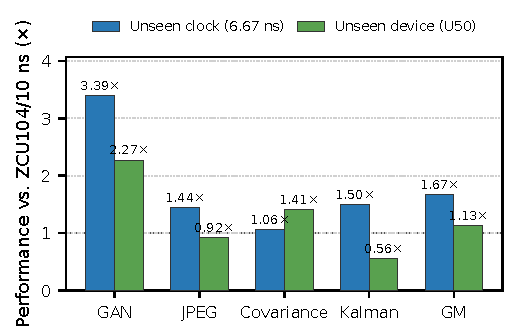
\includegraphics[
        width=0.98\columnwidth
    ]{figures/04_Experimental/target_generalization_zero_shot_qor-1.pdf}
\caption{
    \textbf{Zero-shot generalization to unseen deployment targets.}
    Starting from ZCU104/10\,ns, the frozen SALT-HLS latency policy is
    evaluated at an unseen 6.67\,ns clock and on an unseen U50 FPGA
    without retraining. Performance is normalized to the synthesized
    ZCU104/10\,ns SALT-HLS design using nominal execution time
    (cycles $\times$ requested period); values above $1\times$ indicate
    improvement over the source-target design. GM denotes the geometric
    mean across all four kernels.
}
\Description{
    Grouped bar chart reporting zero-shot performance relative to the
    ZCU104 10-nanosecond source-target SALT-HLS design for GAN, JPEG,
    Covariance, and Kalman. The two series correspond to an unseen
    6.67-nanosecond clock and an unseen U50 FPGA.
    }
    \label{fig:target-generalization}
\end{figure}

Figure~\ref{fig:target-generalization} asks a stricter question than
workload generalization: can the frozen policy respond to a deployment
target that was never observed during training? Starting from
ZCU104/10\,ns, we perturb one target dimension at a time. ZCU104/6.67\,ns
tests interpolation to an unseen clock between the trained 10 and 5\,ns
points, whereas U50/10\,ns changes the FPGA while holding the clock fixed.
The four kernels intentionally expose different target sensitivities.
GAN provides abundant coupled compute/memory parallelism (11 actions);
JPEG is the largest and most control/buffer-rich case (21 actions);
Covariance is a regular static-control kernel with only seven loop
actions; and Kalman has 13 actions, including six array decisions, while
its source-target design already occupies 96.8\% of ZCU104 BRAM. We retain
Kalman despite its negative U50 result precisely to expose the difficult
memory-constrained regime rather than selecting only favorable transfers.

The metric is execution-time improvement relative to the synthesized
ZCU104/10\,ns SALT-HLS design, not speedup over a pragma-free target
baseline. All four kernels benefit at the unseen clock, giving a
$1.67\times$ geometric mean. The mechanisms nevertheless differ:
GAN improves by $3.39\times$, as latency falls from 2,839 to 1,255 cycles
in addition to the shorter period; Kalman retains essentially the same
cycle count and therefore obtains the expected $1.50\times$ frequency
gain; JPEG tolerates a small cycle increase and still reaches
$1.44\times$; while Covariance grows from 59,643 to 84,671 cycles, nearly
cancelling the faster clock and yielding only $1.06\times$. Thus clock
transfer is useful but not equivalent to simply multiplying performance
by frequency: the HLS schedule and operator implementation may themselves
change under a different timing constraint.

Cross-device transfer is harder. U50 improves GAN and Covariance by
$2.27\times$ and $1.41\times$, respectively, but JPEG reaches
$0.92\times$ and Kalman $0.56\times$, giving a $1.13\times$ geometric
mean. The failures are informative rather than synthesis anomalies.
JPEG uses more aggressive parallelism on U50 yet increases DSP/FF/LUT
from 779/36.8K/116.1K to 1,159/60.2K/155.5K without reducing cycle
latency. Kalman similarly reorganizes its memory hierarchy but increases
latency from 327,772 to 589,818 cycles. Zero-shot device transfer
therefore does not guarantee that additional hardware parallelism matches
the kernel's actual bottleneck.


\paragraph{Directive response.}
The directives explain the asymmetric transfer behavior. At 6.67\,ns,
51 of the 52 action decisions remain unchanged; only one JPEG pipeline
decision changes. The intermediate timing target is therefore handled
largely by a portable source-target policy and by target-aware HLS
scheduling. U50 instead changes 17/52 actions (32.7\%). On GAN, SALT-HLS
doubles the cyclic banking of the two hidden-layer buffers
($15/25\!\rightarrow\!30/50$) together with the corresponding unroll
factors, a coherent memory/compute scaling that accompanies the
$2.27\times$ gain. JPEG raises two unroll factors from $2$ to $8$,
increases \texttt{QuantBuff} banking from $2$ to $8$, and completely
partitions two additional buffers, but this extra parallelism does not
translate to lower latency. Covariance requires no directive change and
still gains $1.41\times$, showing that its regular policy transfers
directly. Kalman changes 8/13 actions, doubling several partition and
unroll factors, yet performance regresses; its high source-target memory
pressure makes the useful hardware organization strongly device
dependent.

Overall, the experiment shows that target conditioning provides useful
zero-shot portability, but not universal target optimality. Frequency
interpolation is robust across all four workloads, whereas device transfer
depends more strongly on whether the source-level parallelization strategy
remains appropriate for the new hardware. The negative JPEG and Kalman
cases therefore delimit the zero-shot capability and motivate the
target-specific adaptation evaluated next.



\subsubsection{Post-Route Validation}
\label{subsubsec:postroute-validation}

Finally, we place and route all 12 designs underlying
Fig.~\ref{fig:target-generalization} with Vitis/Vivado 2021.1.
Table~\ref{tab:postroute-targets} reports the post-route critical-path
period. All designs fit the target FPGA and meet their requested clock,
including the unseen-target configurations.

\begin{table}[t]
    \centering
    \caption{\textbf{Post-route timing of the zero-shot designs (ns).}
    Column headers give the requested period; every reported period is
    below its corresponding target.}
    \label{tab:postroute-targets}
    \scriptsize
    \setlength{\tabcolsep}{3.2pt}
    \renewcommand{\arraystretch}{1.03}

    \begin{tabular}{lccc}
        \toprule
        & \textbf{ZCU104} & \textbf{ZCU104} & \textbf{U50} \\
        \textbf{Kernel}
        & \textbf{10 ns}
        & \textbf{6.67 ns}
        & \textbf{10 ns} \\
        \midrule
        GAN        & 6.289 & 4.830 & 6.908 \\
        JPEG       & 9.418 & 6.570 & 9.211 \\
        Covariance & 7.989 & 5.600 & 9.012 \\
        Kalman     & 8.381 & 6.238 & 9.097 \\
        \bottomrule
    \end{tabular}
\end{table}

This physical validation sharpens the interpretation of
Fig.~\ref{fig:target-generalization}. In particular, the negative U50
transfers for JPEG (0.92$\times$) and Kalman (0.56$\times$) still close
timing at 9.211 and 9.097\,ns, respectively. Their regressions therefore
come from increased cycle latency rather than failure to meet the target
clock. Conversely, all four unseen 6.67\,ns designs close timing---the
tightest is JPEG at 6.570\,ns---confirming that the observed
cross-frequency gains correspond to physically realizable implementations.
Post-route timing is used here as a feasibility check; performance remains
normalized using cycles times the requested period, as in
Fig.~\ref{fig:target-generalization}.



\subsubsection{Few-shot Adaptation to Uknown Device}

\EV{Include if good results sep 9 morning}


\subsection{Comparison with State-of-the-Art}
\label{subsec:sota-comparison}


\begin{figure*}[t]
    \centering
    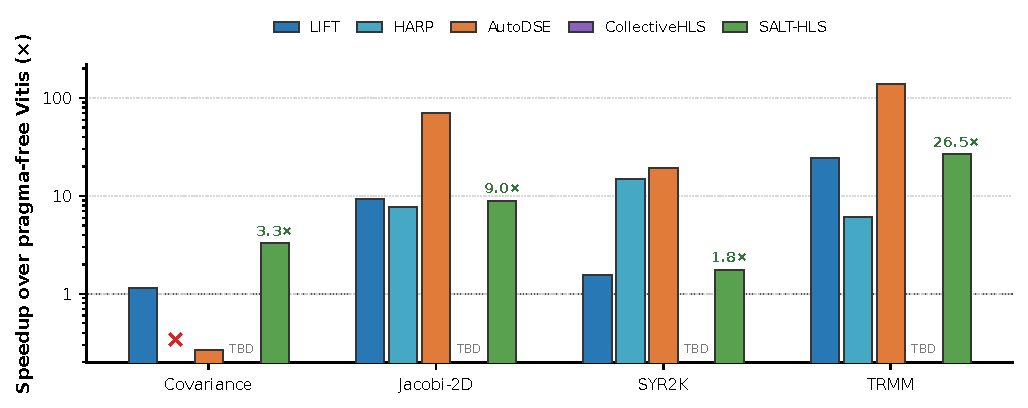
\includegraphics[
        width=0.82\textwidth
    ]{figures/04_Experimental/sota_common_kernels-2.pdf}
    \caption{
        \textbf{Comparison with state-of-the-art HLS optimization
        approaches on the common PolyBench kernels.}
        Speedup is measured over the same pragma-free Vitis baseline.
        A red $\times$ denotes a method for which no feasible synthesized
        design is available; ``n/e'' denotes a method--kernel pair not
        evaluated in the corresponding experiment, while ``TBD'' reserves
        the CollectiveHLS result currently being evaluated.
    }
    \Description{
        Grouped logarithmic bar chart comparing LIFT, HARP-DSE, AutoDSE,
        CollectiveHLS, and SALT-HLS on Covariance, Jacobi-2D, SYR2K,
        and TRMM.
    }
    \label{fig:sota-common}
\end{figure*}


\begin{figure}[t]
    \centering
    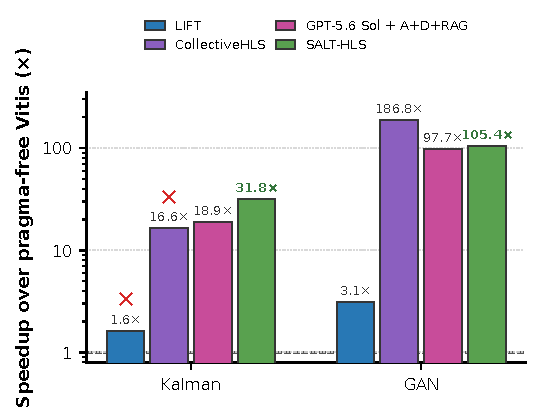
\includegraphics[
        width=0.98\columnwidth
    ]{figures/04_Experimental/sota_gan_kalman-3.pdf}
    \caption{
        \textbf{Comparison on fully unseen applications.}
        We compare SALT-HLS with LIFT, CollectiveHLS, and the strongest
        general-purpose LLM baseline, GPT-5.6 Sol under
        action-, domain-, and retrieval-augmented prompting.
        Speedup is measured over the pragma-free Vitis baseline.
        Red $\times$ markers denote synthesized configurations that violate
        FPGA resource constraints.
    }
    \Description{
        Logarithmic grouped bar chart comparing LIFT, CollectiveHLS,
        GPT-5.6 Sol with action-domain-RAG prompting, and SALT-HLS on
        the Serrano Kalman filter and GAN.
    }
    \label{fig:sota-external}
\end{figure}

\paragraph{Optimization Cost}


\begin{table}[t]
    \centering
    \caption{\textbf{Online optimization cost.}
    HLS calls used to guide optimization are separated from
    synthesis used only to validate the final selected design.
    Offline dataset construction and model training are excluded.}
    \label{tab:optimization-cost}

    \scriptsize
    \setlength{\tabcolsep}{2.5pt}
    \renewcommand{\arraystretch}{1.08}

    \begin{tabular}{lcccc}
        \toprule
        \textbf{Method} &
        \textbf{Search} &
        \textbf{HLS$_{\mathrm{fb}}$} &
        \textbf{HLS$_{\mathrm{val}}$} &
        \textbf{Online cost} \\
        \midrule

        AutoDSE~\cite{sohrabizadeh2020autodse}
        & $\sim$200
        & $\sim$200
        & incl.
        & 25\,h/kern. \\

        HARP-DSE~\cite{sohrabizadeh2023harp}
        & $\sim$100k
        & 0
        & 10
        & 1\,h + val. \\

        CollectiveHLS~\cite{ferikoglou2024collectivehls}
        & 1 prop.
        & 0$^\dagger$
        & 1$^\dagger$
        & 3.2\,s + HLS \\

        LIFT~\cite{prakriya2025lift}
        & 1 decode
        & 0
        & 1
        & N/R + HLS \\

        \textbf{SALT-HLS}
        & \textbf{1 decode}
        & \textbf{0}
        & \textbf{1}
        & \textbf{TBD + HLS} \\

        \bottomrule
    \end{tabular}

    \vspace{1pt}
    \parbox{0.98\columnwidth}{\scriptsize
    HLS$_{\mathrm{fb}}$: synthesis calls whose results guide
    configuration selection; HLS$_{\mathrm{val}}$: final
    measurement/validation synthesis.
    ``N/R'' denotes not reported.
    $^\dagger$CollectiveHLS can perform additional HLS calls when
    its directive re-proposal mechanism is activated.}
\end{table}


\subsection{Comparison with State of the Art}
\label{subsec:sota-comparison}

Figures~\ref{fig:sota-common} and~\ref{fig:sota-external} compare
SALT-HLS with complementary HLS optimization paradigms: synthesis-driven
DSE (AutoDSE), surrogate-guided DSE (HARP), direct LLM pragma generation
(LIFT), knowledge-driven transfer (CollectiveHLS), and a strong
general-purpose LLM. The comparison is intentionally split into two
sets because no baseline supports the same source/tool contract on all
applications. AutoDSE and HARP are released around Merlin-compatible
design spaces and databases~\cite{sohrabizadeh2020autodse,
sohrabizadeh2023harp}; we therefore evaluate them on the four common
PolyBench kernels. Their public flows require Merlin-compatible projects,
whereas GAN and Serrano-Kalman are external direct-Vitis applications,
so the latter panel uses baselines that can be applied to these sources.
These are consequently \emph{end-to-end framework comparisons under
each method's native directive space}, rather than a matched-action-space
ablation. AutoDSE's released implementation explicitly requires the
source project to run through Merlin, while HARP builds its DSE database
from AutoDSE/Merlin projects. \cite{sohrabizadeh2020autodse,
sohrabizadeh2023harp}

\paragraph{Common PolyBench kernels.}
Figure~\ref{fig:sota-common} exposes a clear quality--search-cost
trade-off. SALT-HLS reaches $3.29\times$, $8.97\times$,
$1.77\times$, and $24.62\times$ on Covariance, Jacobi-2D,
SYR2K, and TRMM, respectively, from a single generated configuration.
Its strongest relative result is Covariance: LIFT reaches
$1.14\times$, AutoDSE returns a $0.27\times$ configuration, and
HARP produces no feasible design among its physically validated
top-10 surrogate candidates. This case illustrates an advantage of
learning the configuration-selection policy directly: a surrogate
ranking can still concentrate its highest-ranked candidates in an
infeasible region, whereas SALT-HLS is trained from synthesized
target-feasible configurations and conditions the prediction explicitly
on the target resource limits.

The ranking reverses on Jacobi-2D and SYR2K. AutoDSE reaches
$70.32\times$ and $19.13\times$, while HARP reaches $7.64\times$
and $14.76\times$; on TRMM, AutoDSE reaches $139.19\times$,
substantially above both LIFT ($26.54\times$) and SALT-HLS
($24.62\times$). These gaps should not be interpreted as a failure of
structural grounding alone: the methods expose different optimization
spaces. Merlin combines \texttt{PIPELINE}, \texttt{PARALLEL}, and
\texttt{TILE} transformations and can derive lower-level memory
organization from these high-level choices, while SALT-HLS predicts
pipeline, unroll, and explicit array-partition actions learned from
GN$\Omega$SIS. AutoDSE can therefore exploit transformation
combinations that are absent or sparsely represented in SALT-HLS's
training support. This is particularly visible on SYR2K and TRMM,
where the best Merlin configurations use aggressive parallelization,
pipeline flattening, or tiling.

There is a concrete data limitation behind this distinction.
GN$\Omega$SIS represents each loop action by one categorical loop
directive, e.g., \texttt{pipeline\_1} or \texttt{unroll\_$k$}.
An exhaustive audit of our supplied multi-target training export
(1.11M loop-action instances) finds no example in which pipeline and
unroll are simultaneously active at the same action. Thus, although
the SALT-HLS output schema does not forbid such a combination, its
supervision provides no positive example from which to learn it. This
inherited support bias helps explain why search-based Merlin methods can
occasionally discover more aggressive configurations on regular
PolyBench nests. The public GN$\Omega$SIS schema likewise exposes one
loop-specific directive value per loop action. \cite{ferikoglou2026gnomegasis}

\paragraph{External GAN and Kalman applications.}
Figure~\ref{fig:sota-external} tests a different form of generalization:
the optimizers must operate on applications outside the common
PolyBench/Merlin comparison. On GAN, CollectiveHLS is strongest at
$186.8\times$, followed by SALT-HLS at $105.4\times$ and
GPT-5.6 Sol with action/domain/RAG prompting at $97.7\times$;
LIFT reaches $3.1\times$. GAN is a favorable case for transferring
aggressive parallelism: its regular dense computation exposes substantial
independent compute and memory-level parallelism. CollectiveHLS is
specifically designed to transfer directive distributions from
previously characterized applications with similar source-level
properties~\cite{ferikoglou2024collectivehls}, explaining why its
knowledge-based policy can be particularly effective on such a case.
The near-SALT performance of GPT-5.6 Sol is also informative: once
eligible actions, legal domains, and HLS guidance are supplied explicitly,
a strong general-purpose model can recover a competitive configuration
for a regular kernel.

Kalman separates the methods more sharply. SALT-HLS reaches
$31.81\times$ while remaining feasible at 96.8\% BRAM; GPT-5.6 Sol
reaches $18.9\times$, whereas CollectiveHLS ($16.6\times$) and
LIFT ($1.6\times$) exceed the resource limits. This is precisely the
regime in which target conditioning matters: the pragma-free Kalman
design already consumes 97.1\% of ZCU104 BRAM, leaving little tolerance
for an optimization policy that treats resource feasibility only
implicitly. LIFT is trained primarily for latency and explicitly does
not use resource utilization as an input supervision signal; invalid
designs are discouraged indirectly through their performance weight
~\cite{prakriya2025lift}. CollectiveHLS likewise optimizes latency from
transferred historical knowledge and its original evaluation already
identifies Kalman as an unseen-application feasibility failure
~\cite{ferikoglou2024collectivehls}. In contrast, SALT-HLS learns from
component-wise feasible targets and conditions every directive decision
on device, clock, BRAM/DSP/FF/LUT budgets, and objective. Its
action-aligned compiler memory further exposes the loop--memory relations
needed to coordinate unrolling with partitioning under the nearly
saturated BRAM constraint.

\paragraph{What does the comparison establish?}
No single optimizer dominates every kernel. Long-running DSE can exploit
a richer native transformation space and reaches the best latency on
several regular PolyBench kernels; knowledge transfer is exceptionally
strong on GAN. SALT-HLS instead provides a different operating point:
one objective- and target-conditioned directive configuration, no online
HLS feedback, and feasible synthesized outputs across the reported
comparisons. Its advantage is largest when optimization quality depends
on jointly reasoning about program structure and a binding hardware
constraint, as in Covariance and especially Kalman. Conversely, the
SYR2K/TRMM gaps expose an important limitation inherited from the
GN$\Omega$SIS supervision: direct prediction can only learn
transformation combinations adequately represented in its training
support. We therefore interpret SALT-HLS not as replacing exhaustive
search in every regime, but as substantially reducing online optimization
cost while retaining competitive QoR, explicit target awareness, and
robust feasibility across heterogeneous and external applications.




